%%%%%%%%%%%%%%%%%%%%%%%%%%%%%%%%%%%%%%%%%%%%%%%%%%%%%%%%%%%%%%%%%%%
%                                                                 %
%                            CHAPTER FIVE                         %
%                                                                 %
%%%%%%%%%%%%%%%%%%%%%%%%%%%%%%%%%%%%%%%%%%%%%%%%%%%%%%%%%%%%%%%%%%%

\chapter{APPLICATION TO ADAPTIVE SIMULATIONS}
\label{chap:apps}

{\bf attribution of PHASTA active flow and Albany to TOMS paper}

{\bf the Proteus and second Albany example are attributed to the SISC paper}

\section{Workflow Integration}

Introduce how parallel adaptivity fits into workflows.

\section{Proteus}

In collaboration with the U.S. Army Corp of Engineers'
Coastal Hydraulics Laboratory and their Proteus CFD code,
we are using our flexible array structure to enable
coupled mesh adaptation with mesh motion in the face
of fluid-structure interaction with moving objects.
Figure \ref{fig:proteus} shows a mesh of a buoyant object
splashing down inside a tank of water.
Proteus carries out an initial nodal repositioning and
smoothing to track this motion, while adaptivity
guided by error estimates ensure the discretization
error and element quality remain controlled.
The adaptation metric may also be anisotropic, as shown
in Figure \ref{fig:proteus_aniso}.

\begin{figure}
\begin{center}
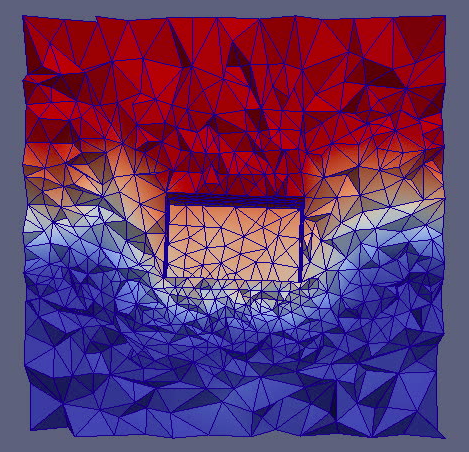
\includegraphics[width=0.4\textwidth]{proteus.png}
\caption{Floating object fluid-structure-interaction adaptivity}
\label{fig:proteus}
\end{center}
\end{figure}

\begin{figure}
\begin{center}
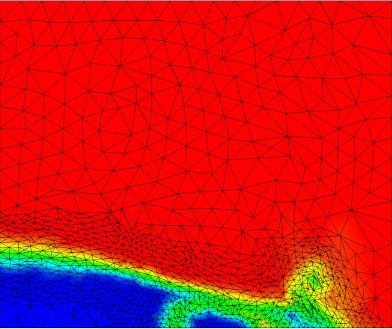
\includegraphics[width=0.6\textwidth]{proteus_aniso.png}
\caption{Anisotropic mesh near fluid boundary}
\label{fig:proteus_aniso}
\end{center}
\end{figure}

\section{Alexa}

\begin{figure}[t]\vspace*{4pt}
\centerline{
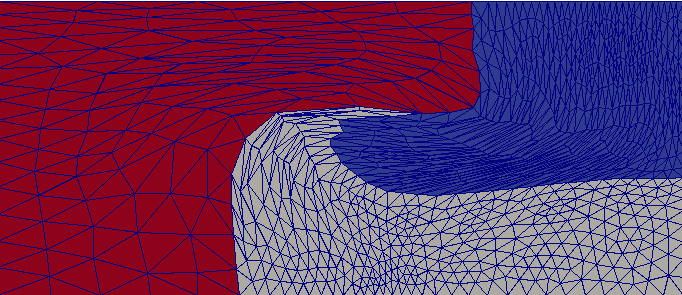
\includegraphics[width=0.5\textwidth]{tpp_noadapt.png}
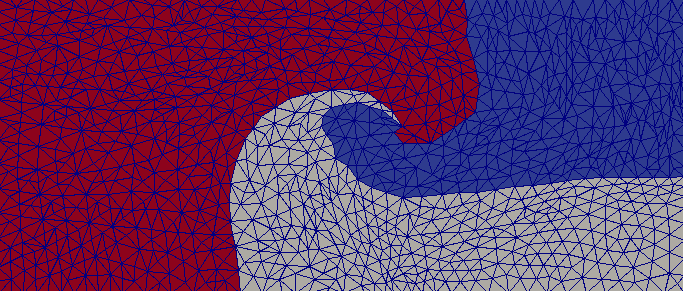
\includegraphics[width=0.5\textwidth]{tpp_adapt.png}}
\caption{Triple point problem: (left) purely Lagrangian
(right) Lagrangian with adaptation}\vspace*{-6pt}
\label{fig:tpp}
\end{figure}

In collaboration with Sandia National Laboratories, an
experimental shock hydrodynamics application is being developed
to explore the benefits of using a Lagrangian formulation with
adaptivity and mesh motion.
Figure \ref{fig:tpp} shows one of our early test cases,
a triple point problem \cite{del2011metric}.
The figure compares the solution with and without adaptation
included in the workflow.
When adaptation is included, it is attempted after every explicit
time step.
Given the small amount of nodal motion per time step, relative
to element sizes, each adaptivity call should be making very
minimal changes to the topology and solution, if any.
The code can proceed quickly without rebuilding any structures
if no mesh modification is deemed necessary after a given time step.
For the triple point case, the adaptive workflow required
7722 time steps to reach the point ($t=4$) in Figure \ref{fig:tpp}.
The non-adaptive workflow required 105,832 time steps (a 14X increase over the adaptive workflow)
due to better element quality.
We are just starting to develop the proper size field controls
for this kind of application and its validation is ongoing
work beyond the scope of this thesis.
We have also developed solution transfer methods for cavity operators
that satisfy certain properties, such as conservation of
mass and momentum.
Continued development of transfer methods is important for bringing adaptivity to
a wider range of applications.

\section{PHASTA Active Flow Control}
\label{sec:phasta_active}

PHASTA \cite{JanWhi99,WhiJanDey2003} is an effective implicit finite element
based CFD code for bridging a broad range of time and length scales in various
flows including turbulent ones (based on URANSS, DES, LES, DNS). It has been
applied with anisotropic adaptive algorithms \cite{Sahn06,Sahn07,Sahn08,
ovcharenko2013parallel}
along with advanced numerical models of flow physics
\cite{HugLES99,TeJaSUPG,TeJaDFWR2}. Modeling large-scale aerodynamic problems
and active flow control's effects on large-scale flow changes (for instance,
re-attachment of separated flow or virtual aerodynamic shaping of lifting
surfaces) from micro-scale input \cite{Amitay:98,Glezer:02,Sahni:11} requires an
efficient parallel adaptive workflow.

\begin{figure}
\begin{center}
\begin{scriptsize}
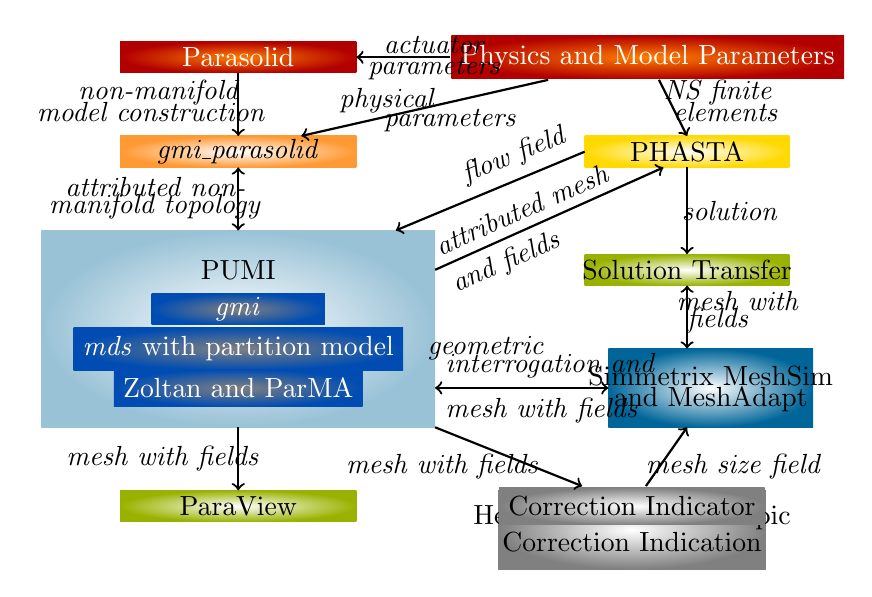
\begin{tikzpicture}%[decoration={bent,aspect=.3}]
\shade[outer color=blue!60!green!40, inner color=white] (-1.5,0) rectangle
(3.5,2.5);
\shade[outer color=orange!60!green, inner color=white] (-.5,-1.2) rectangle
(2.5,-.8);
\node at (1,-1)    {ParaView};
\shade[outer color=blue!70!green, color=white] (-.1,1.3) rectangle (2.1,1.7);
\node [color=white] at (1, 1.5)    {\emph{gmi}};
\node[rectangle, outer color=blue!70!green, color=white, thick] at (1, 1)
{\emph{mds} with partition model};
\node[rectangle, outer color=blue!70!green, color=white, thick] at (1, 0.5)
{Zoltan and ParMA};
\node at (1, 2) {PUMI};
\shade[outer color=red!70!black, inner color=orange] (-.5,4.5) rectangle
(2.5,4.9);
\node [color=white] at (1,4.7)    {Parasolid};
\node[rectangle, outer color=red!70!black, inner color=orange, color=white,
thick] (B) at (6.2,4.7) {Physics and Model Parameters};
\shade[outer color=orange!80, inner color=white] (-.5,3.3) rectangle (2.5,3.7);
\node at (1,3.5)    {\emph{gmi\_parasolid}};
%\node[rectangle, outer color=orange!30!yellow, inner color=white, thick] (D) at
%(6.7,3.5) {Mesh-based Analysis};
\shade[outer color=orange!30!yellow, inner color=white] (5.4,3.3) rectangle
(8,3.7);
\node at (6.7,3.5)     {PHASTA};
%\node[rectangle, outer color=orange!60!green, inner color=white, thick] (E) at
%(6.7,2) {Solution Transfer};
\shade[outer color=orange!60!green, inner color=white] (5.4,1.8) rectangle
(8,2.2);
\node at (6.7,2)     {Solution Transfer};
\shade[outer color=blue!60!green, inner color=white] (5.7,0) rectangle (8.3,1);
\node at (7, .65) {Simmetrix MeshSim};
\node at (7, .35) {and MeshAdapt};
%yellow!60!blue
\shade[outer color=blue!50!yellow, inner color=white, thick] (4.3,-1.8)
rectangle (7.7,-.8);
\node at (6, -1.15) {Hessian-based Anisotropic};
\node at (6, -1.45) {Correction Indication};
%(A)
%physics and model parameters -> input domain definition
\draw[->,decorate,thick] (B)--(2.5,4.7);
\node at (3.5, 4.85)   {\emph{actuator}};
\node at (3.5, 4.55)   {\emph{parameters}};
%physics and model parameters->complete domain definition
\draw[->,decorate,thick] (B)--(1.8,3.7);
\node at (2.9, 4.15)   {\emph{physical}};

\node at (3.7, 3.9)   {\emph{parameters}};
%physics and model parameters->mesh-based analysis
\draw[->,decorate,thick] (B)--(6.7,3.7);
\node at (7.1, 4.25)   {\emph{NS finite}};
\node at (7.2, 4)   {\emph{elements}};
%(B)
%input domain definition->complete domain definition
\draw[->,decorate,thick] (1,4.5)--(1,3.7);
\node at (0, 4.25)   {\emph{non-manifold}};
\node at (-.1, 4)   {\emph{model construction}};
%(C)
%complete domain definition<->PI
\draw[<->,decorate,thick] (1,3.3)--(1,2.5);
\node at (-.05, 3.05)   {\emph{attributed non-}};
\node at (-.05, 2.8)   {\emph{manifold topology}};
%(D) mesh based analysis->PI
\draw[->,decorate,thick] (5.4,3.5) node[above left, rotate=22]{\emph{flow
field}} to (3,2.5);
%PI->mesh based analysis
\draw[->,decorate,thick] (3.5,2) node[above right, rotate=24]{\emph{attributed
mesh}} node[below right,rotate=24] {\emph{and fields}} to (6.4, 3.3);
%mesh-based analysis -> solution transfer
\draw[->,decorate,thick] (6.7,3.3) -- (6.7,2.2);
\node at (7.25, 2.75)    {\emph{solution}};
%PI<->mesh adaptation
\node at (4.15,1) {\emph{geometric}};
\draw[<->,decorate,thick] (3.5,.5) node[above right]{\emph{interrogation and}}
node[below right]{\emph{mesh with fields}}  to (5.7,.5);
%mesh adaptation<->solution transfer
\draw[<->,decorate,thick] (6.7,1.8)--(6.7,1);
\node at (7.35, 1.6)    {\emph{mesh with}};
\node at (7.1, 1.35)    {\emph{fields}};
%PI->postprocessing
\draw[->,decorate,thick] (1,0) -- (1,-.8); \node at (.05, -.4)    {\emph{mesh
with fields}};
\node[rectangle, outer color=blue!50!yellow, inner color=white, thick] (H) at
(6,-1) {Correction Indicator};
%PI->Correction indicator
\draw[->,decorate,thick] (3.5,0) -- (H);
\node at (3.6, -.5)    {\emph{mesh with fields}};
%Correction indicator->adaptation
\draw[->,decorate,thick] (H) -- (6.7,0);
\node at (7.3, -.5)    {\emph{mesh size field}};
\end{tikzpicture}
\end{scriptsize}
\end{center}
\caption{Workflow of parallel PHASTA adaptive loop}
\label{fig:phastaWorkflow}  \end{figure}

\begin{figure}
\centering
\begin{tabular}{cc}
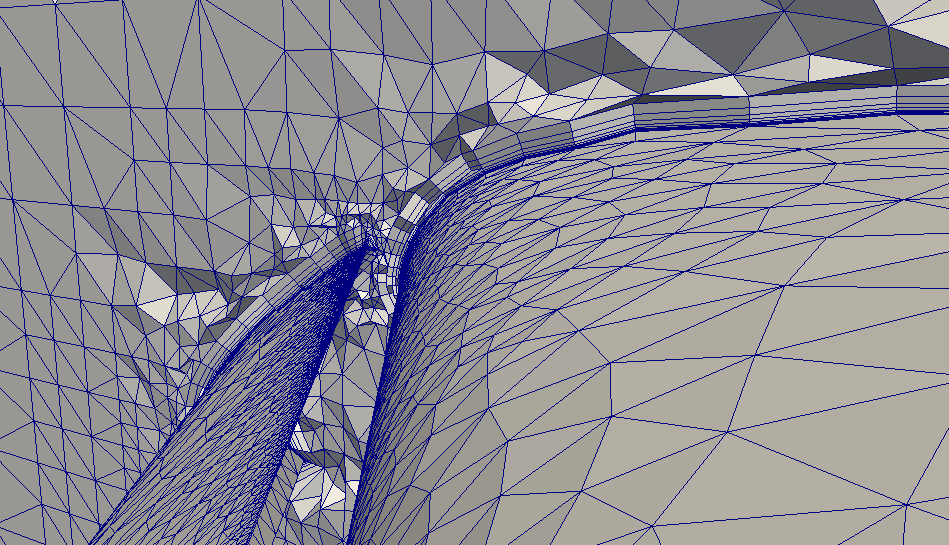
\includegraphics[width=2.5in]{TrapWing_Cut_LeadingEdge_Init.png}&
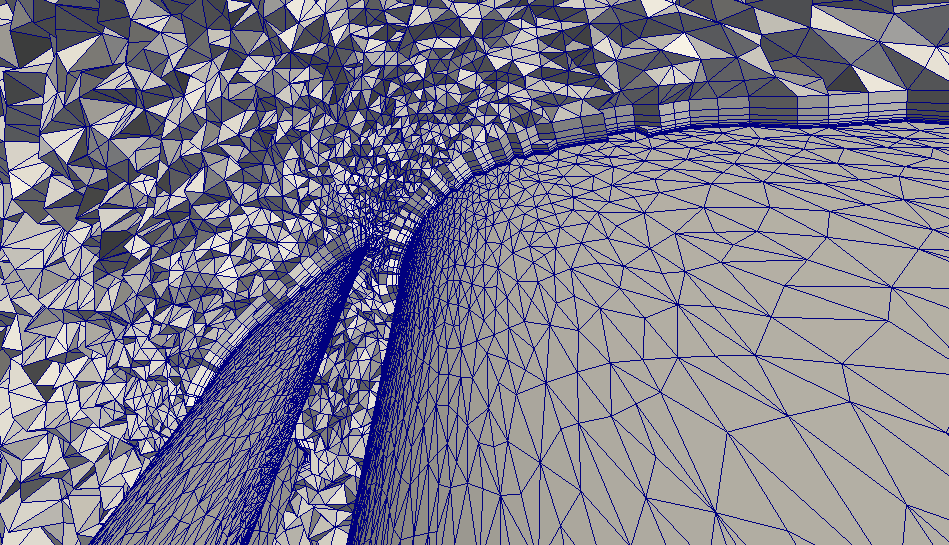
\includegraphics[width=2.5in]{TrapWing_Cut_LeadingEdge_Adapt2.png}
\end{tabular}
\caption{Cut views of the initial (left) and adapted (right) anisotropic
boundary layer meshes for NASA TrapWing~\cite{chitale-aiaa14}}
\label{fig:phasta-mesh}  % the \label command comes AFTER the caption
\end{figure}

A workflow supporting parallel adaptive PHASTA flow simulations is illustrated in
Figure \ref{fig:phastaWorkflow}.
Figure \ref{fig:phasta-mesh} shows the initial
and adapted mesh near the leading edge of TrapWing NASA test
case \cite{chitale-aiaa14}.
The Argonne Leadership Computing Facility's IBM
BlueGene Q Mira system provides 4 hardware threads per core.
Running this workflow in Mira system with 4 MPI processes per core,
PHASTA achieved strong scaling
in mesh-based computations on up to 786,432 cores using 3,145,728 MPI processes
with a 92 billion element mesh \cite{rasquinCise2014}.

Key to this scaling and the efficiency of the workflow is controlling the load
balance through PUMI interfaces to Zoltan and ParMA load balancing and
partitioning tools. The workflow invokes load balancing after parallel mesh
generation, during general unstructured mesh adaptation and before execution of
PHASTA. Dynamic partitioning using a combination of ParMA and Zoltan is executed
after parallel mesh generation to reach the partition sizes needed by mesh
adaptation and PHASTA.  During mesh adaptation, ParMA predictive load balancing
procedures are used to ensure system memory is not exhausted and the resulting
mesh is balanced.  Lastly, before PHASTA execution, ParMA multi-criteria
diffusive procedures are run to reduce both the mesh element and mesh vertex
imbalance.  During each of these stages the association of PHASTA solution data
with mesh entities is maintained via field migration and local solution
transfer procedures.

An in-memory coupling supporting a parallel adaptive PHASTA analysis
loop \cite{smith2016building} using the components depicted in
Figure \ref{fig:phastaWorkflow} is enabled through a functional interface to the
FORTRAN 77/90 based flow solver. Through the use of FORTRAN 2003
\emph{iso\_c\_bindings}, this interface supports interoperability with C/C++
components and supports the control of solver execution, and the interrogation
and management of solver data structures.

\section{Albany Adaptive Loop}

Albany \cite{albany14} is a general-purpose finite element code built on the
Trilinos framework \cite{TrilinosOverview,trilinosweb}, both of which are developed
primarily at Sandia National Laboratories. This code is highly extensible,
allowing the creation of new finite element numerical methods, which makes it an
ideal platform for research in finite elements. The design of Albany is parallel
from the start, and also includes an abstract interface for discretization
storage, i.e. a mesh database, as well as various adaptivity codes.

As illustrated in Figure \ref{fig:albanyWorkflow}, PUMI was used to form a
parallel adaptive loop using Albany and MeshAdapt \cite{smith2016building,meshadaptweb}.
This is entirely an in-memory coupling: the mesh database provides simple
connectivity arrays and field data arrays to Albany for analysis, which Albany
returns after a specified number of analysis steps on an unchanging mesh.

Once the data is back in PUMI structures, mesh adaptivity can be invoked on them
to produce a new mesh, and solution transfer of key solution variables allows
this new state to be sent back to Albany for further analysis,
resulting in a self-contained, in-memory adaptive finite element code. The rich
encoding of the PUMI mesh means that it is almost always a superset of the mesh
information required for an analysis code. As such, we were able to convert not
only to connectivity structures used internally by Albany, but also to another
mesh data structure known as STK, part of the Trilinos framework. This makes
PUMI more interoperable with any finite element codes involving the Trilinos
framework. Figure \ref{fig:albany-mesh} illustrates the initial and adapted mesh
in large deformation analysis with Albany adaptive loop.

We are also using the MDS array structure to manage very large meshes
in a compact and scalable way for a different Albany simulation
studying the mechanical properties of computer circuitry.
Figure \ref{fig:ibm} shows how the initial
meshes used for this project represent
multiple CAD model regions with graded resolution.
The initial mesh is further refined and partitioned,
and runs have exceeded one billion elements, utilizing
up to 4 racks (65536 cores) of an IBM BlueGene/Q computer.
The memory use of our structure is quite small compared
to the storage used for the stiffness matrix and
Krylov vectors in this problem.

\begin{figure}
\centering
\begin{tabular}{cc}
  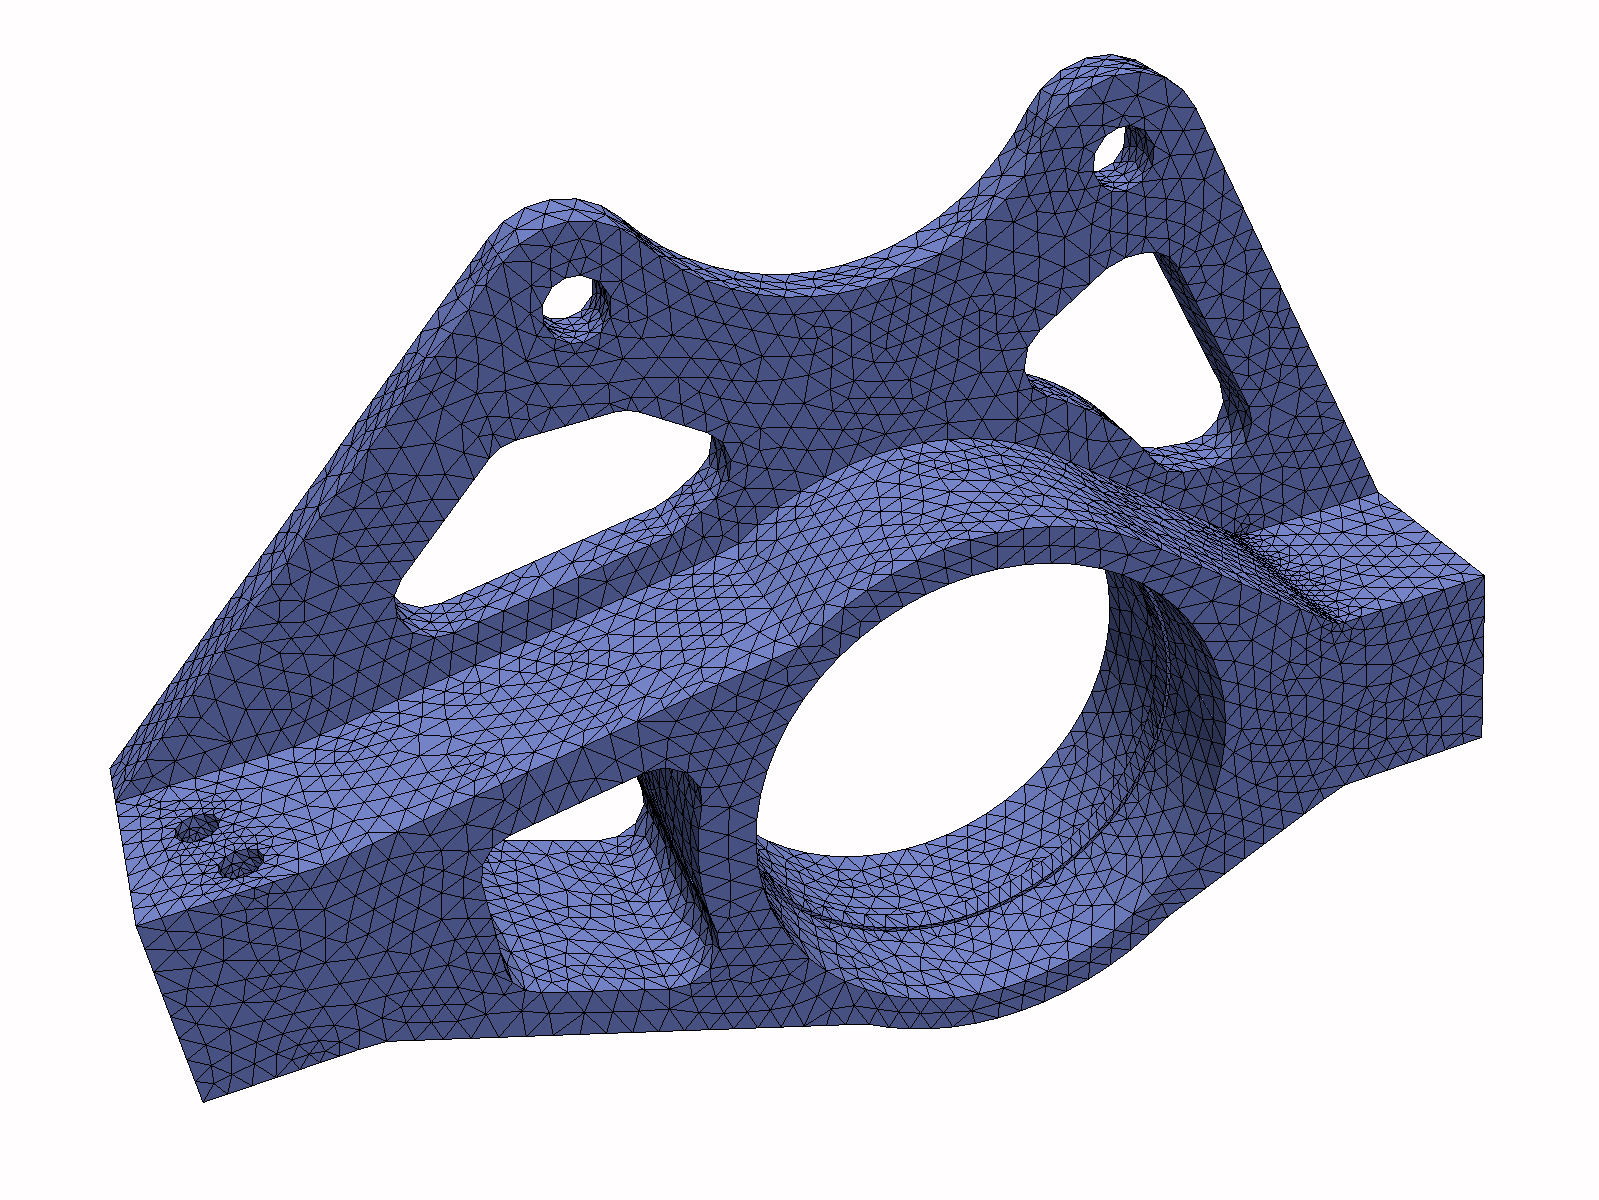
\includegraphics[width=.5\textwidth]{albany1.png}&
  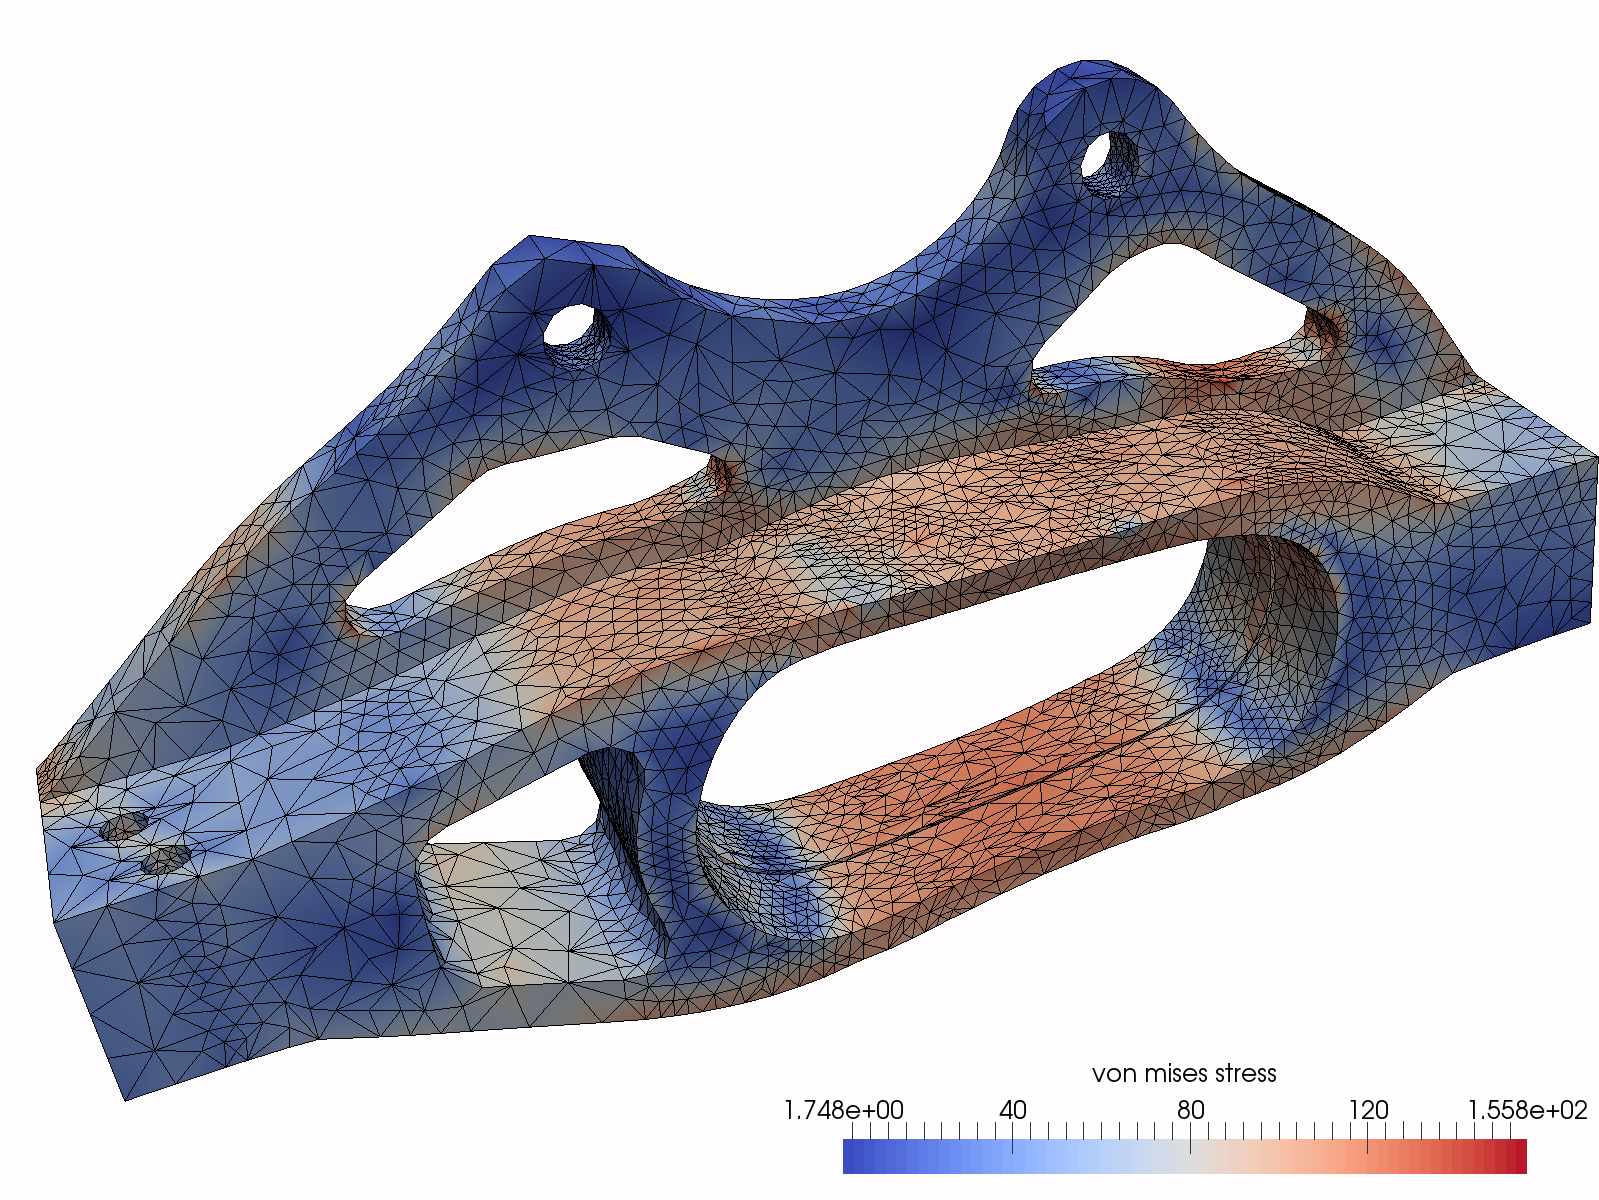
\includegraphics[width=.5\textwidth]{albany2.png}
\end{tabular}
\caption{Initial (left) and adapted mesh showing the Von Mises stress field that
guides adaptivity (right)} \label{fig:albany-mesh}
\end{figure}

\begin{figure}
\begin{center}
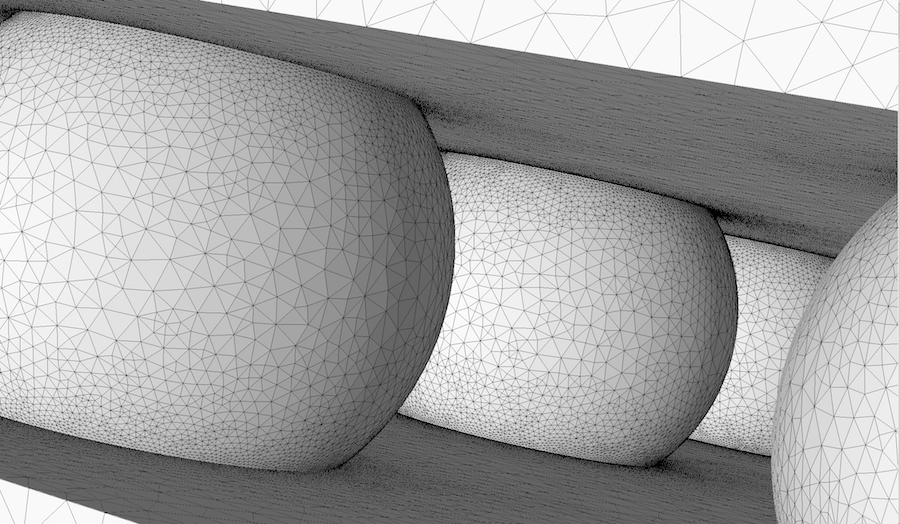
\includegraphics[width=0.6\textwidth]{ibm.png}
\caption{Graded multi-material mesh to initiate large scale runs}
\label{fig:ibm}
\end{center}
\end{figure}

\begin{figure}
\begin{center}
\begin{scriptsize}
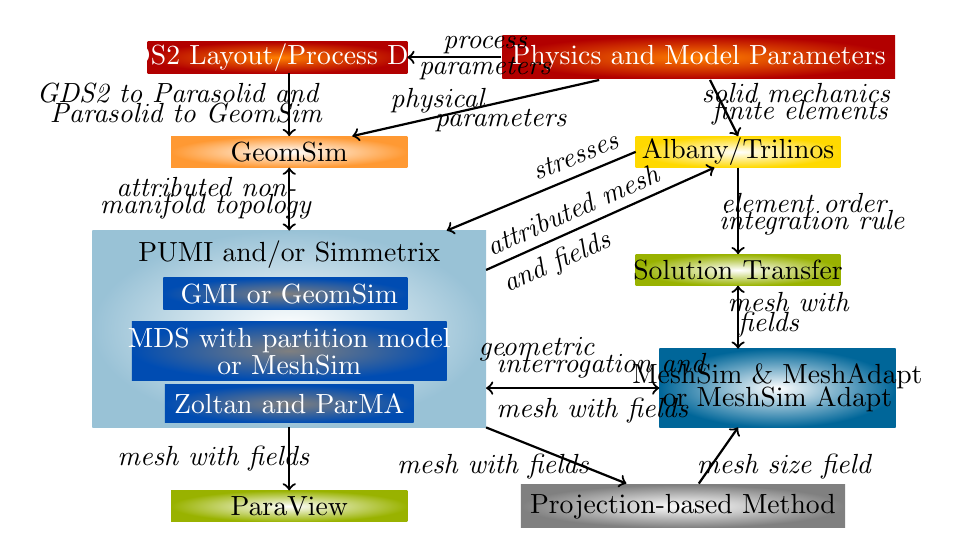
\begin{tikzpicture}%[decoration={bent,aspect=.3}]
\shade[outer color=blue!60!green!40, inner color=white] (-1.5,0) rectangle
(3.5,2.5);
%\node[rectangle,outer color=orange!60!green, inner color=white, thick] (G) at
%(1,-1) {Postprocessing/Visualization};
\shade[outer color=orange!60!green, inner color=white] (-.5,-1.2) rectangle
(2.5,-.8);
\node at (1,-1)    {ParaView};
\shade[outer color=blue!70!green, color=white] (-.6,1.5) rectangle (2.5,1.9);
\node [color=white] at (1, 1.7)    {GMI or GeomSim};
\shade[outer color=blue!70!green, color=white] (-1,.6) rectangle (3,1.35);
\node[color=white] at (1, 1.1) {MDS with partition model};
\node[color=white] at (1, .8) {or MeshSim};
\node[rectangle, outer color=blue!70!green, color=white, thick] at (1, 0.3)
{Zoltan and ParMA};
\node at (1, 2.2) {PUMI and/or Simmetrix};
\shade[outer color=red!70!black, inner color=orange] (-.8,4.5) rectangle
(2.5,4.9);
\node [color=white] at (.85,4.7)    {GDS2 Layout/Process Data};
\node[rectangle, outer color=red!70!black, inner color=orange, color=white,
thick] (B) at (6.2,4.7) {Physics and Model Parameters};
\shade[outer color=orange!80, inner color=white] (-.5,3.3) rectangle (2.5,3.7);
\node at (1,3.5)    {GeomSim};
%\node[rectangle, outer color=orange!30!yellow, inner color=white, thick] (D) at
%(6.7,3.5) {Mesh-based Analysis};
\shade[outer color=orange!30!yellow, inner color=white] (5.4,3.3) rectangle
(8,3.7);
\node at (6.7,3.5)     {Albany/Trilinos};
%\node[rectangle, outer color=orange!60!green, inner color=white, thick] (E) at
%(6.7,2) {Solution Transfer};
\shade[outer color=orange!60!green, inner color=white] (5.4,1.8) rectangle
(8,2.2);
\node at (6.7,2)     {Solution Transfer};
\shade[outer color=blue!60!green, inner color=white] (5.7,0) rectangle (8.7,1);
\node at (7.2, .65) {MeshSim \& MeshAdapt};
\node at (7.2, .35) {or MeshSim Adapt};
%yellow!60!blue
\node[rectangle, outer color=blue!50!yellow, inner color=white, thick] (H) at
(6,-1) {Projection-based Method};
%(A)
%physics and model parameters -> input domain definition
\draw[->,decorate,thick] (B)--(2.5,4.7);
\node at (3.5, 4.85)   {\emph{process}};
\node at (3.5, 4.55)   {\emph{parameters}};
%physics and model parameters->complete domain definition
\draw[->,decorate,thick] (B)--(1.8,3.7);
\node at (2.9, 4.15)   {\emph{physical}};
\node at (3.7, 3.9)   {\emph{parameters}};
%physics and model parameters->mesh-based analysis
\draw[->,decorate,thick] (B)--(6.7,3.7);
\node at (7.45, 4.25)   {\emph{solid mechanics}};
\node at (7.5, 4)   {\emph{finite elements}};
%(B)
%input domain definition->complete domain definition
\draw[->,decorate,thick] (1,4.5)--(1,3.7);
\node at (-.4, 4.25)   {\emph{GDS2 to Parasolid and}};
\node at (-.3, 4)   {\emph{Parasolid to GeomSim}};
%(C)
%complete domain definition<->PI
\draw[<->,decorate,thick] (1,3.3)--(1,2.5);
\node at (-.05, 3.05)   {\emph{attributed non-}};
\node at (-.05, 2.8)   {\emph{manifold topology}};
%(D) mesh based analysis->PI
\draw[->,decorate,thick] (5.4,3.5) node[above left, rotate=22]{\emph{stresses}}
to (3,2.5);
%PI->mesh based analysis
\draw[->,decorate,thick] (3.5,2) node[above right, rotate=24]{\emph{attributed
mesh}} node[below right,rotate=24] {\emph{and fields}} to (6.4, 3.3);
%mesh-based analysis -> solution transfer
\draw[->,decorate,thick] (6.7,3.3) -- (6.7,2.2);
\node at (7.55, 2.85)    {\emph{element order}};
\node at (7.65, 2.6)    {\emph{integration rule}};
%PI<->mesh adaptation
\node at (4.15,1) {\emph{geometric}};
\draw[<->,decorate,thick] (3.5,.5) node[above right]{\emph{interrogation and}}
node[below right]{\emph{mesh with fields}}  to (5.7,.5);
%mesh adaptation<->solution transfer
\draw[<->,decorate,thick] (6.7,1.8)--(6.7,1);
\node at (7.35, 1.6)    {\emph{mesh with}};
\node at (7.1, 1.3)    {\emph{fields}};
%PI->postprocessing
\draw[->,decorate,thick] (1,0) -- (1,-.8); \node at (.05, -.4)    {\emph{mesh
with fields}};
%PI->Correction indicator
\draw[->,decorate,thick] (3.5,0) -- (H);
\node at (3.6, -.5)    {\emph{mesh with fields}};
%Correction indicator->adaptation
\draw[->,decorate,thick] (H) -- (6.7,0);
\node at (7.3, -.5)    {\emph{mesh size field}};
\end{tikzpicture}
\end{scriptsize}
\end{center}
\caption{Workflow of parallel Albany adaptive loop}
\label{fig:albanyWorkflow}
\end{figure}
